
\chapter{度量与分析}

\hypertarget{a-kjux6b65ux9aa4}{%
\subsection{A: KJ步骤}\label{a-kjux6b65ux9aa4}}

\emph{一种头脑风暴方法,每人把自己想法写在便利贴上,一起轮流把所有便利贴排放分组}

\begin{enumerate}
\tightlist
\item
  把主题以问题形式写在大白纸的头顶;
\item
  把相关的事实写在便利贴上面,用黑色;
\item
  搜集相关的事实,如果是一组人的话,分散到不同人手上;
\item
  (团队)查看描述是否不清楚,是否要整理?
\item
  每人轮流把相关的便利贴组合在一起;
\item
  当每人都已经调整过便利贴组合后,一起把每一组便利贴加上一个题目,用红色标识;
\item
  红色的标题下包含相关事实的内容;
\item
  把相关的红色题目(最好不超过3个)组合在一起;
\item
  给这大组一个题目 -- 蓝色;
\item
  在题目下放上相关的红色小组;
\item
  把蓝色的题目和剩下红色的小组或单独没有分类的便利贴都在墙上放好,也可以用一些箭头描述它们的因果关系;
\item
  (可选)
\end{enumerate}

\begin{description}
\item[]
\begin{description}
\tightlist
\item[]
A 投票看看哪个是最重要的红色组

B 也可以加些总结性的描述
\end{description}
\end{description}

\hypertarget{a-ux5982ux4f55ux753bimrux63a7ux5236ux56fe}{%
\subsection{A:
如何画ImR控制图}\label{a-ux5982ux4f55ux753bimrux63a7ux5236ux56fe}}

1/ 计算单值(X)平均数 (X-bar)\\
2/ 计算移动极差(mR moving Range)均值\\
3/ 利用以下方程式,计算X的上下限\\
::UNPL=X-bar+(2.66*mR均值)\\
::LNPL=X-bar -(2.66*mR均值)\\
4/ 利用以下方程,计算移动极差的上限\\
::URL=3.27* mR均值\\
5/ 如果X或mR有超出范围,表示有过程变化的信号,过程不稳定\\
6/ 也不应该有连续8个或以上的点都持续提升,因这种发生的概率低于百分之一\\
Note:

\begin{description}
\item[]
\begin{description}
\tightlist
\item[]
UNPL=Upper Natural Process Limit

LNPL=Lower Natural Process Limit

URL=Upper Range Limit
\end{description}
\end{description}

例子:\\


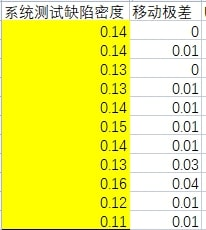
\includegraphics[width=10cm]{微信截图_20210929131748.jpg}

1/ 计算单值(X)平均数 (X-bar) (X-bar)=0.135\\
2/ 计算移动极差(mR moving Range)均值 如第一移动极差为0;
第二移动极差为0.01;10点的均值=0.0128\\
3/ 计算X的上下限: UCL=0.170 LCL =0.100\\
4/ 计算移动极差的上限 使用上面公式 UCL=0.042 LCL =0\\
5/ 在2图中加上这些上下限与平均线:


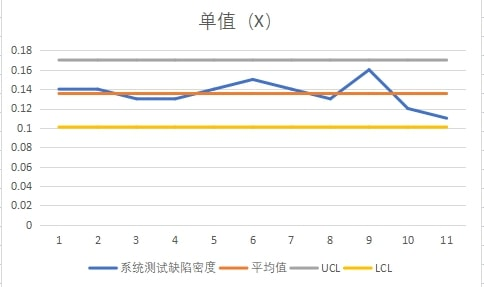
\includegraphics[width=10cm]{微信截图_20210927084548.jpg}


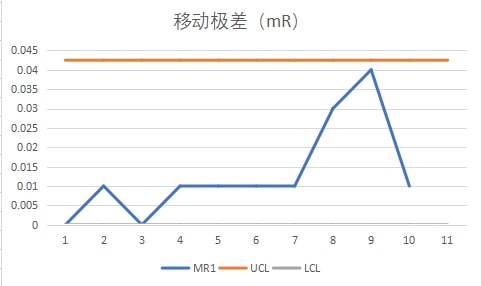
\includegraphics[width=10cm]{微信截图_20210927084434.jpg}

\hypertarget{aux6c34ux6676ux7403ux8499ux5730ux5361ux7f57ux9884ux6d4bux6a21ux578b}{%
\subsection{A:水晶球蒙地卡罗预测模型}\label{aux6c34ux6676ux7403ux8499ux5730ux5361ux7f57ux9884ux6d4bux6a21ux578b}}

\begin{itemize}
\tightlist
\item
  按每个过程的统计数据,估计对应缺陷排除百分比的上下限与均值,工作量也类似。例如,从公司基线,代码走查的缺陷排除率是55\%左右;评审总工作量(不包含修正缺陷)大概为20人时。如果开始时没有充足的项目数据,可以先依据行业基线:如代码正式审查应能排除85\%,但平均人时会增加到35人时
  (也是不包含修正缺陷)。得出下图:
\end{itemize}


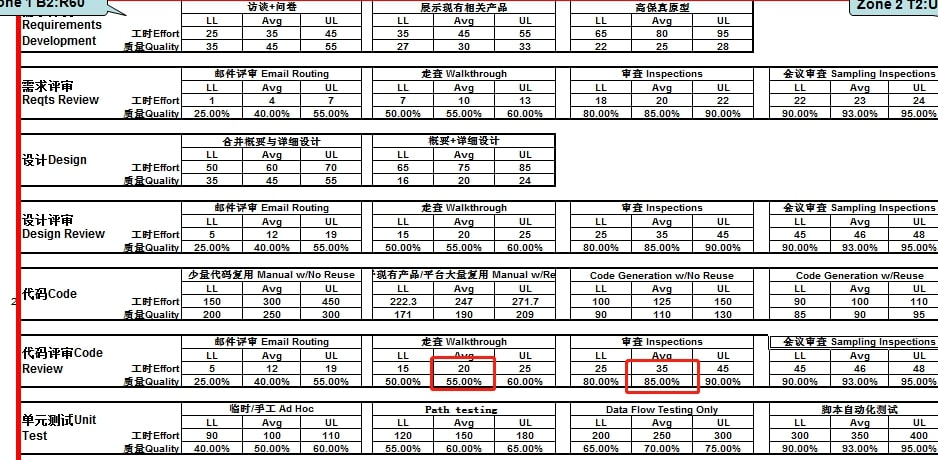
\includegraphics[width=10cm]{微信截图_20211027011246.jpg}

\begin{itemize}
\tightlist
\item
  模型会自动按输入的最大最小值计算标准差,变成分布(如:正态(normal)分布、三角形(triangular)分布),水晶球模型会依据黄格里的数字选取对应的分布,
\end{itemize}


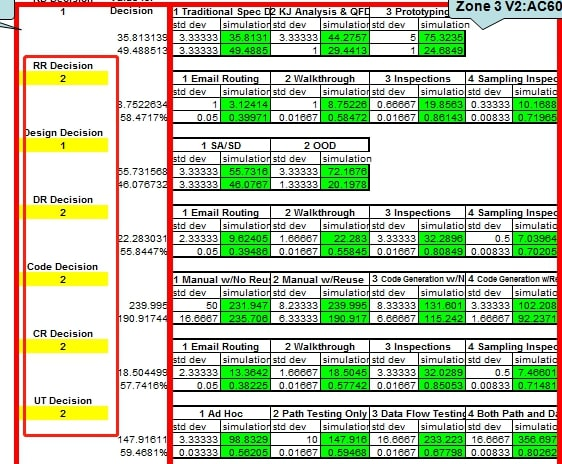
\includegraphics[width=10cm]{微信截图_20211027011403.jpg}

\begin{itemize}
\tightlist
\item
  取对应的分布,依据项目历史数据统计,估算各个过程缺陷的返工工作量与成本。例如:修复一个系统测试发现的缺陷,平均要用6000元,最高7500,最低5000。如果缺陷导致的如果是工时那行,填上对应工种的平均人时总成本。水晶球模型就会依据我们输入的范围估算单位成本的分布,放在绿格里。
\end{itemize}


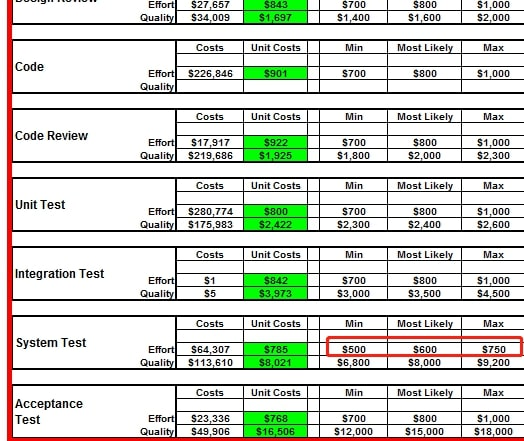
\includegraphics[width=10cm]{微信截图_20211027012006.jpg}

\begin{itemize}
\tightlist
\item
  如果从需求到验收测试,每一个过程的成本数都是单一值; 我们可以简单用 XLS
  把数加起来得出总数。但如果每个过程的成本数都是一个分布,例如三角形分布,
\end{itemize}

必须要使用蒙地卡罗方法才可以把每个过程''加''起来。

\begin{itemize}
\tightlist
\item
  水晶球可以帮我们估计质量成本的分布,例如我们需求评审用审查(2),设计评审用走查(2)
  ,代码评审也用走查(2),单元测试是手工(1),系统测试估计走3轮(2),验收测试预计走3轮(2),水晶球就会依据我们刚刚输入的分布用蒙地卡罗预测模型预估质量成本的分布。
\end{itemize}


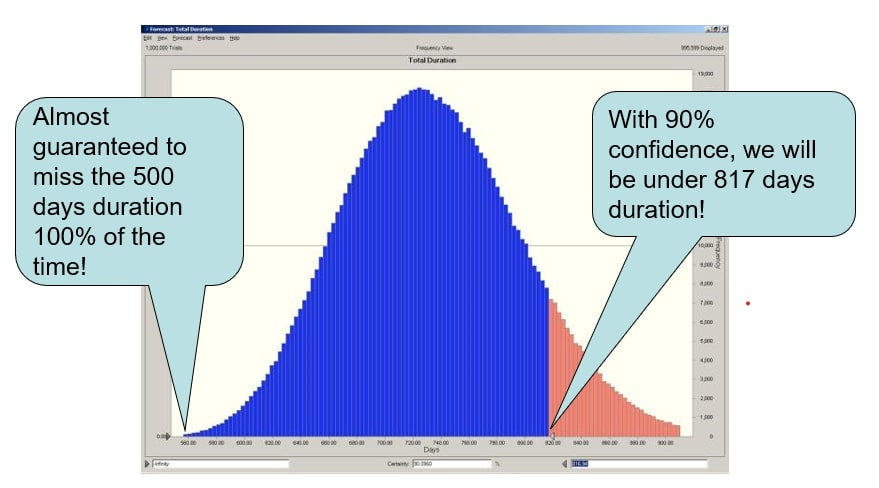
\includegraphics[width=10cm]{HmttDistScreenshot_2021-10-08_165836.jpg}

\begin{itemize}
\tightlist
\item
  比较各种不同的配搭,选出质量成本最低是哪个配搭组合,帮助项目组在策划时选择使用什么方法,得出最佳效果。
\end{itemize}

下图显示一直水晶球优化的过程,和最终的最``佳''配搭:\\


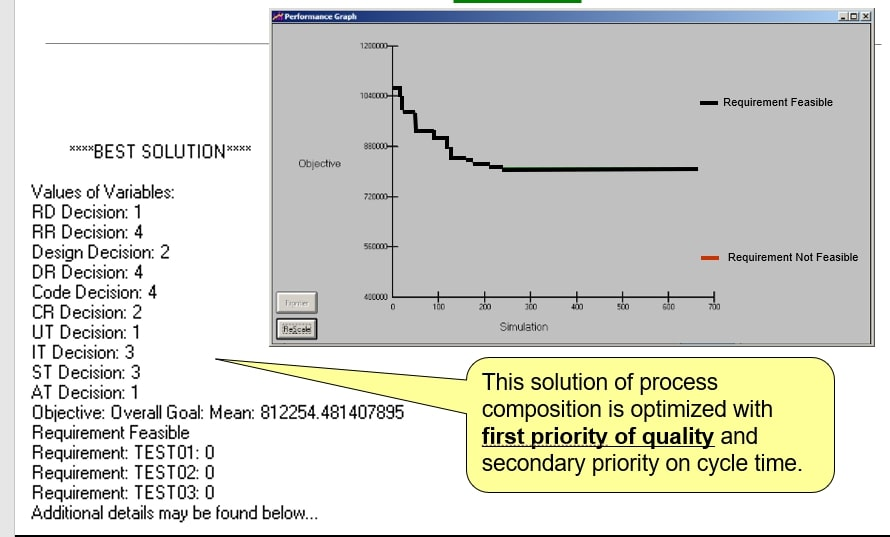
\includegraphics[width=10cm]{HmttOptScreenshot_2021-10-08_165653.jpg}

在需求评审,设计评审,代码评审,单元测试,系统测试,验收测试都有两种选择时,跑优化,95\%的置信区间
得出 Overrall goal (Quality + Effort) = 1476773


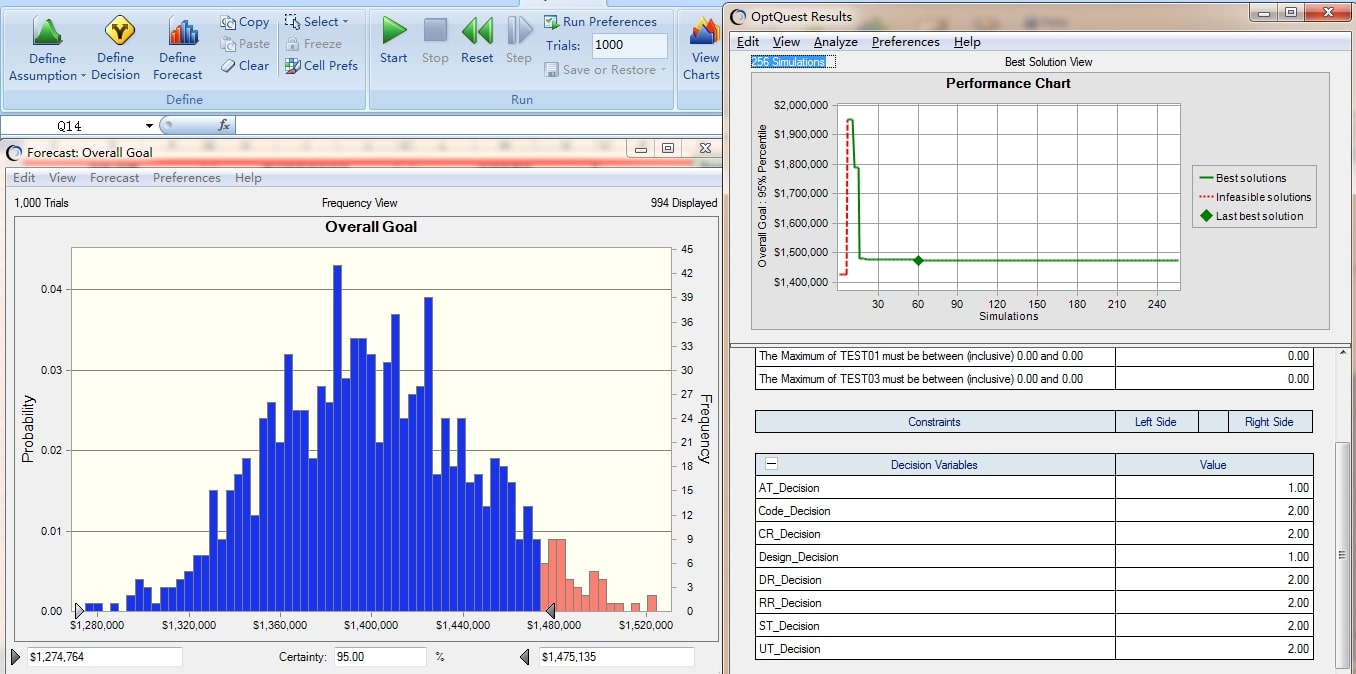
\includegraphics[width=10cm]{微信截图_20211103023018.jpg}


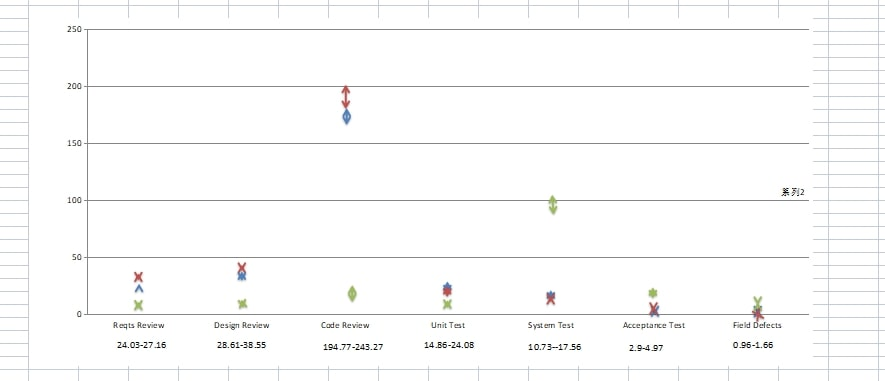
\includegraphics[width=10cm]{微信截图_20211118145154.jpg}